% Ray: market-level forecasting (results). Pairs with 3b_level_methods.tex.
% Table I, the macro and rolling-origin numbers, and the figure's data:
% scripts/report_level_eval.py, written to outputs/report_level/. Figure:
% figures/level_backtest.png. The numbers with block premiums (1.5, 5.8, 0.5, 1.7,
% -65 to -9, 591.2 and 594.0) come from notebooks/2_models.ipynb, Part 2.3.

\subsection{Market-Level Forecasts}
\label{sec:level-results}

\begin{table}[htbp]
\caption{Level forecasts on the holdout period, using the tuned LightGBM of Section~\ref{sec:holdout}, without block premiums and without level weighting. Bias is mean prediction minus actual rent in dollars, at 1--3 and 13--15 months ahead.}
\begin{center}
\begin{tabular}{|l|r|r|r|}
\hline
\textbf{Level forecast} & \textbf{RMSE} & \textbf{Bias +1--3} &
\textbf{Bias +13--15} \\
\hline
Month index in tree     & 487.5 & $4.9$   & $-61.8$ \\
Hold                    & 484.4 & $19.0$  & $-46.9$ \\
Damped trend            & 483.9 & $31.4$  & $29.8$ \\
\textbf{Average}        & \textbf{483.5} & $25.2$ & $-8.7$ \\
Straight line           & 634.6 & $109.6$ & $643.9$ \\
\hline
Oracle (not usable)     & 484.9 & $27.2$  & $59.2$ \\
\hline
\end{tabular}
\label{tab:level-holdout}
\end{center}
\end{table}

RMSE alone hides the drift. For this model with the month index, RMSE falls
from 528 at 1--3 months ahead to 461 at 13--15, partly because later rents are
less spread out, while its bias grows from $+\$5$ to $-\$62$.

Forecasting the level removes most of that drift
(Table~\ref{tab:level-holdout}): the average forecast lowers RMSE from 487.5 to
483.5 and the bias at 13--15 months to $-\$9$. The bias result carries over to the
model with block premiums of Section~\ref{sec:lightgbm} ($-\$65$ to $-\$9$), but
most of the RMSE gain does not: there the average gains 1.5 on the holdout and 5.8
on the tuning split. Hold gains 3.1 in Table~\ref{tab:level-holdout}, but only 0.5
with premiums, and it is 1.7 worse on the tuning split. It is also about level
with the month index across the rolling origins below, so the decomposition alone
is not a general gain. The straight line over-predicts by \$644 by the end, as
expected.

Hold, damped trend and average are all within \$1.5 of the oracle, and the
average even scores below it. On the holdout period the tree's premiums run
about 1\% high, so the oracle level over-predicts by \$42 on average. The
average forecast, lagging a market still edging up, sits about 1\% below the
oracle level and happens to offset it. Across origins the oracle is best on
average.

The macroeconomic alternative fails our test. On the tuned model, adding COE
alongside the month index raises RMSE from 488 to about 530 (507 to 557 over five
seeds, so a single run is not reliable). COE fell in early 2024 to levels last
seen in early 2022, when median rent was about \$800 lower. The damage comes with
the tuned settings: with the same columns and an earlier untuned configuration,
COE scores 488.5 against 491.1. Replacing the month index with COE also fails, at
683.9 against 652.7 with no time feature at all, on that earlier configuration.
Share indices score 490 alongside the month index, level with the placebo (489),
and most of them leave their training range during the test months, where a tree
cannot follow them. In no setup does a macro series do meaningfully better than a
share price with no link to rent, so we drop them.

\begin{figure}[htbp]
\centerline{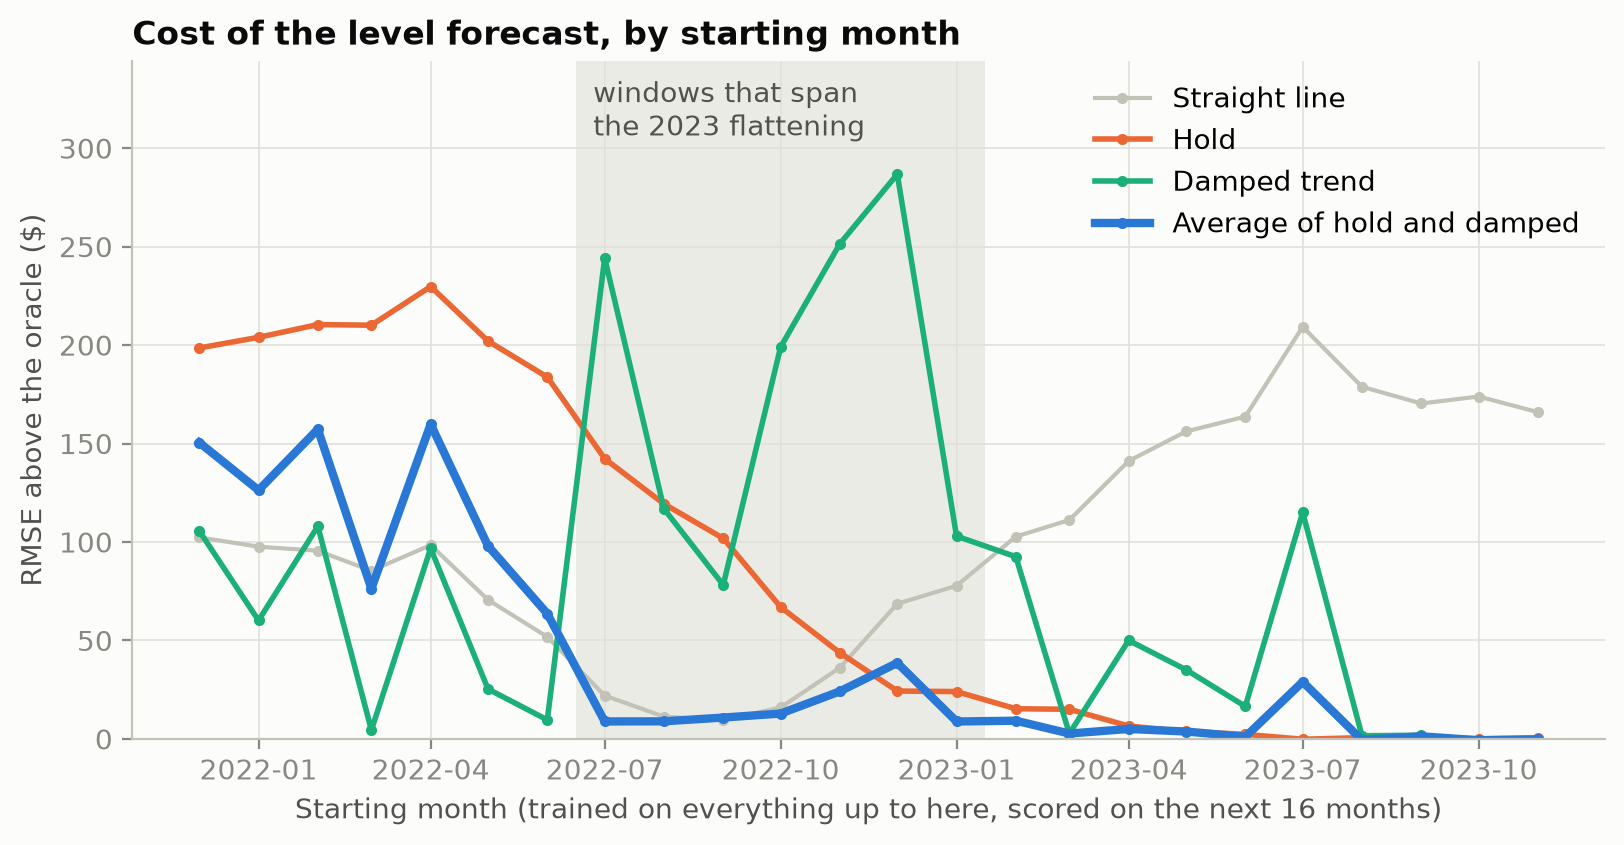
\includegraphics[width=\columnwidth]{figures/level_backtest.png}}
\caption{RMSE above the oracle by forecast origin, each scoring the next 16
months, for the model of Table~\ref{tab:level-holdout}. Gaps below zero are shown as zero. Hold fails during the climb, and damped trend at origins before the 2023
flattening (shaded).}
\label{fig:level-backtest}
\end{figure}

The holdout period cannot separate hold, damped trend and average, but the
rolling-origin evaluation can (Fig.~\ref{fig:level-backtest}). They fail at
opposite times. From origins during the climb (December 2021 to June 2022),
hold is the worst of the four forecasts at every origin, \$184 to \$230 above the
oracle, because it freezes a rising market. From the seven origins up to a year
before the flattening, damped trend is the worst in five, up to \$287 above,
because it carries the climb's slope into a market that has stopped. Across
origins the average costs \$41 above the oracle on average, against \$83 to \$101
for the others, and \$160 at its worst origin, against \$209 to \$287. It is
therefore the safest forecast when the market may turn. Its weakness is the climb
itself, where it trails damped trend by \$45 to \$73 because it inherits half of
hold's lag.

That advantage comes from origins before the flattening. Over the ten origins from
February 2023, whose market resembles the one at the end of training, the average
(531.5) has no edge over hold (530.9). On the tuning split with premiums, damped
trend (591.2) also beats the average (594.0). The local evidence therefore shows
insurance against a turn in the market, not a clear gain in a flat one.

A test submission that changed only the level scored 439.7 on the public leaderboard, against 436.8 for the model
we submit (Section~\ref{sec:lightgbm}), so that model stays on the month index, and we treat the
market level as a known limitation. No local split can observe the test months,
so this is the one choice in this report made on a test score, and one public
score is thin evidence.

These results have four limits. First, neighbouring origins share 15 of their
16 scored months, so they are not independent tests, and the history holds only
one climb and one flattening. Second, the tuned settings were searched for the
model with the month index on data up to December 2023, and are reused
unchanged for the level forecasts and for every origin, including origins
earlier than the data they were tuned on. Third, the rolling origins use the
model without block premiums, so they only suggest how the submitted model would
behave. Fourth, the average was added after seeing an earlier comparison across
three origins, so the size of its gain is optimistic, and this evaluation confirms
that choice more than it makes it.
